% generated by make_combined.py from stage3_real_artifacts/stage3.tex; do not edit
\section{Stage 3 --- Real artifacts across modalities}\label{sec:stage3}

\stagebox{\textbf{In one sentence.} With real, unedited artifacts --- hair in dermoscopy, calipers in thyroid and
ovarian ultrasound, debris in capsule endoscopy --- ROI masking helps far more when the artifact lies outside the ROI
than inside it: the crossover is positive in \sThreeNXPos{} of \sThreeNRuns{} cohort--encoder pairs and in all four
pre-specified location tests after Holm correction; the dermatology encoder DermLIP and, with the radiograph encoder
RAD-DINO, real chest-radiograph devices are the exceptions, and the hair shortcut turns out to be carried largely by correlates of hair rather than by its
pixels.}
\subsection{Where this stage starts}
Stage~1 showed with real hair (E13) that masking harms when hair lies on the lesion and helps when it lies beside it.
Stage~2 established the location law with synthetic artifacts whose position was controlled, in five modalities, and
identified its mechanism (retention with amplified reliance). Synthetic artifacts answer \emph{whether} location can
matter; they cannot show that it matters for the artifacts clinicians actually produce, whose location is set by the
workflow and read from masks. This stage builds real-artifact traps in three more cohorts, validates the automatic
artifact masks that define ``inside'' and ``outside'', replicates across encoder families, asks what actually carries
the hair shortcut, and examines chest radiography, where the law might not hold.

\subsection{Questions}
\begin{enumerate}[label=\textbf{Q3\alph*},leftmargin=*]\itemsep1pt
\item With real artifacts and the same protocol, is ROI masking less useful --- or harmful --- when the artifact lies
inside the ROI than when it lies outside it (a positive crossover)?
\item Does this hold across modalities, artifacts and encoder families?
\item Are the artifact masks that define inside and outside good enough to support the answer?
\item What carries a real shortcut: the artifact's pixels, or things that go with the artifact?
\end{enumerate}
\paragraph{Design: two traps sharing one artifact-free group} A real artifact's location is fixed by the image, so it
cannot be moved. Each cohort is split into images whose artifact lies mostly inside the ROI ($r\ge0.5$, Trap~A) and
images whose artifact lies outside it ($r<0.1$, Trap~B); images with $0.1\le r<0.5$ belong to neither trap. Each trap is
completed by the \emph{same} artifact-free images and receives the environments of Stage~1. This is the E13 design of
Stage~1, which replaced the pilot's overlap-contrast design (E12) because in E12 location itself was the label proxy.
\paragraph{Why these cohorts} Each has (i) an artifact that clinicians produce and that is associated with the
diagnosis through the workflow (calipers are placed on nodules that are measured; debris is more frequent on some lesion
types), (ii) public ROI masks or boxes, (iii) a way to locate the artifact without manual annotation, and (iv) enough
images for an artifact-free group. Table~\ref{s3:tab:rejected} lists the cohorts that failed one of these conditions.

\subsection{Methods}
\subsubsection{Cohorts}
\begin{itemize}[leftmargin=*]\itemsep1pt
\item \textbf{Dermoscopy} --- ISIC 2019 \citep{combalia2019bcn,tschandl2018ham} as in Stage~1: published semi-automatic
hair masks \citep{wegley2026artifacts}; lesion masks from HAM10000 or the U-Net trained on ISIC 2018 Task~1
\citep{codella2019isic}; leakage groups lesion identifier $\cup$ perceptual hash.
\item \textbf{Thyroid ultrasound} --- TN3K images \citep{gong2021tn3k} with TNCD benign/malignant labels (3,493
images, 1,210 malignant) and manual nodule masks. Calipers located by a rule-based detector (dotted measurement lines =
$\ge7$ evenly spaced bright dots; ``+'' calipers by template matching), tuned on 36 images and frozen before its final
audit. $A=0$: no detected caliper pixel; $A=1$: $\ge15$ detected pixels. Groups: pHash $\le8$ (TN3K publishes no
patient identifiers).
\item \textbf{Ovarian ultrasound} --- MMOTU OTU\_2d \citep{zhao2022mmotu} (CC BY 4.0): benign cystic lesions (chocolate
cyst, serous cystadenoma, simple cyst) versus lesions with a solid component (teratoma, theca cell tumour, mucinous
cystadenoma, high-grade serous carcinoma); normal ovaries excluded (1,202 images). The frozen thyroid detector,
unchanged. Groups: pHash $\le8$.
\item \textbf{Capsule endoscopy} --- SEE-AI \citep{seeai2023} (CC BY 4.0), single-class frames: erosion versus
polyp-like lesions; ROI = union of the expert lesion boxes. Contamination (debris, bubbles, bile) masks from the
published expert masks where available (22 frames) and otherwise from a linear probe on DINOv2 patch tokens trained on
2,160 expert-masked frames. $A=0$: contamination $<3\%$ of the frame; $A=1$: $\ge10\%$. Groups: blocks of 100
consecutive frame numbers $\cup$ pHash $\le2$ (no video identifiers are published).
\item \textbf{Chest radiography} --- NIH ChestX-ray14 \citep{wang2017chestxray8}; lungs from a PSPNet
\citep{cohen2022xrv}. (i) \emph{Device traps}: images linked to RANZCR-CLiP device annotations; Trap~A = central venous
catheter inside the lungs, Trap~B = endotracheal tube outside them; four findings with $\ge40$ reversed-test positives;
restricted to AP films (intubated patients are imaged supine, so view could not be matched). (ii) \emph{Chest drains}:
29,687 pneumothorax-labelled images; drains from NEATX human labels and a drain detector (precision 0.95); drains lie
inside the lungs, so this is an in-ROI trap only. Patient-grouped folds.
\end{itemize}
\paragraph{Protocol} Frozen encoders: DINOv2 ViT-B/14 @518 for every cohort; MedSigLIP-448 (a medical vision--language
model) for thyroid, ovary and capsule; ConvNeXt-Base @384 (a CNN) for thyroid and capsule; DermLIP for dermoscopy;
RAD-DINO for chest radiographs. Logistic heads chosen on clean validation data; 5 seeds (42, 123, 456, 789, 2026)
$\times$ 5 grouped folds, fold predictions pooled per seed. Within each label the artifact-bearing images are
subsampled to the source mix of the artifact-free group (source matching; vacuous for single-source cohorts). Gates
fixed before fitting: every matched cell $\ge25$ images and $\ge40$ reversed-test positives. Arms as in Stage~1.
\paragraph{Statistics} Crossed seed$\times$image bootstrap, 10,000 replicates; the crossover's interval resamples the
same images in both traps. The four location tests (P1, one per cohort, DINOv2) are Holm-corrected; everything else is
reported with unadjusted 95\% intervals.

\subsection{Experiments}
\begin{table}[H]\centering\scriptsize
\caption{Experiments of this stage with registration status, the registration document (\texttt{docs/PREREGISTRATION\_<name>.md}), its first commit and the support criterion stated in advance. Commit times are set by the committing machine and are not independent proof of order.}\label{s3:tab:exp}
\begin{tabular}{p{3.1cm}p{2.1cm}p{2.4cm}p{3.2cm}p{3.3cm}}\toprule
Experiment & Status & Registration & First commit (local time) & Support criterion \\\midrule
Dermoscopy hair traps (E13, DINOv2) & \ok{} registered & ISIC2019\_\allowbreak{}TRAPS & \texttt{76e25d4}, 2026-09-26 13:14 & crossover CI $>0$ \\
Dermoscopy hair, DermLIP & \ok{} registered & ISIC2019\_\allowbreak{}TRAPS & \texttt{76e25d4}, 2026-09-26 13:14 & crossover CI $>0$ \\
Thyroid caliper traps & \ok{} registered & THYROID\_\allowbreak{}TRAPS & \texttt{ea57661}, 2026-09-26 22:46 & crossover CI $>0$ \\
Ovarian caliper traps & \ok{} registered & OVARY\_\allowbreak{}TRAPS & \texttt{2517600}, 2026-09-27 07:29 & crossover CI $>0$ \\
Capsule debris traps & \ok{} registered & CAPSULE\_\allowbreak{}TRAPS & \texttt{fcbf8d9}, 2026-09-27 00:40 & crossover CI $>0$ \\
Chest-radiograph device traps & \ok{} registered & CXR\_\allowbreak{}DEVICE\_\allowbreak{}TRAPS & \texttt{4d1a924}, 2026-09-26 18:07 & crossover CI $>0$ \\
Location tests P1 (four cohorts, Holm) & \mixed{} each test registered; Holm grouping post hoc & STATISTICAL\_\allowbreak{}PLAN & \texttt{4e9d44c}, 2026-09-27 09:37 & Holm $p<0.05$, positive estimate \\
Chest drains (NIH) & \ok{} registered & CXR\_\allowbreak{}DRAIN & \texttt{3d0cffc}, 2026-09-27 03:29 & mask $-$ ERM reported with CI, no direction \\
Crossed-bootstrap intervals (A1) & \ok{} registered & FINAL (A1) & \texttt{c45d482}, 2026-09-28 00:35 & a claim is stated only if its crossed CI excludes 0 \\
\bottomrule\end{tabular}
\end{table}


\subsection{Results}
\subsubsection{Cohorts and artifact masks}
\begin{table}[H]\centering\scriptsize
\caption{Real-artifact cohorts and pool sizes (images, positive/negative diagnosis) before the environments are sampled. Trap A: artifact mostly inside the ROI ($r\ge0.5$); Trap B: outside ($r<0.1$); both share the artifact-free group.}\label{s3:tab:cohorts}
\resizebox{\linewidth}{!}{\begin{tabular}{p{3.4cm}p{2.4cm}p{2.5cm}p{2.2cm}ccc}\toprule
Cohort & Task & Artifact (mask source) & ROI & Artifact-free pos/neg & Trap A pos/neg & Trap B pos/neg \\\midrule
ISIC 2019 dermoscopy (HAM10000, BCN20000, MSK) & melanoma vs other & hair (published masks) & lesion: HAM manual / U-Net & 157/706 & 942/2655 & 969/4412 \\
TN3K ultrasound, TNCD labels & malignant vs benign nodule & calipers (rule detector) & nodule (manual) & 749/1052 & 292/858 & 99/227 \\
MMOTU 2D ultrasound & solid-component vs cystic tumour & calipers (rule detector) & tumour (manual) & 178/170 & 276/341 & 103/91 \\
SEE-AI capsule endoscopy & erosion vs polyp-like lesion & debris (patch probe) & lesion box (expert) & 343/164 & 412/404 & 1009/231 \\
\bottomrule\end{tabular}}
\end{table}

\begin{figure}[H]\centering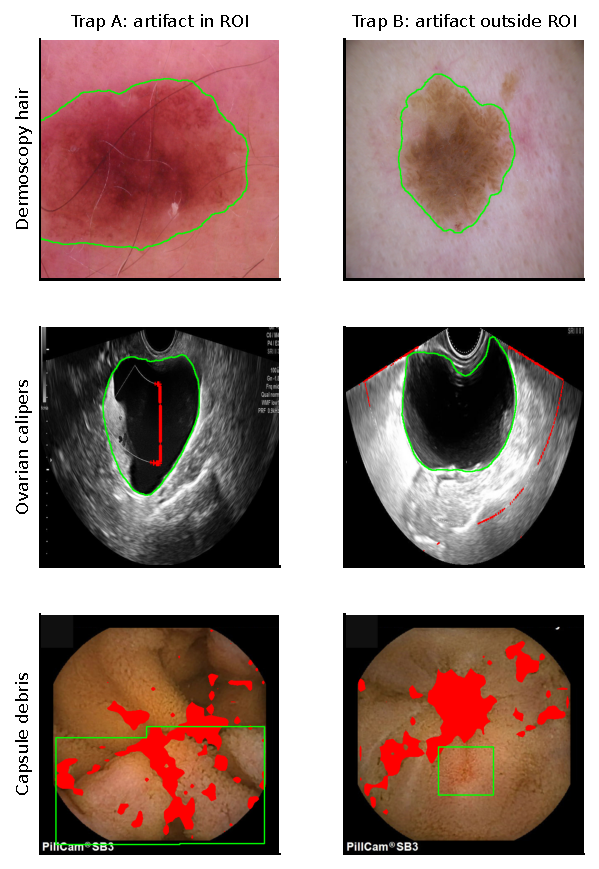
\includegraphics[width=0.60\linewidth]{../stage3_real_artifacts/figures/real_examples.pdf}
\caption{Real artifacts inside (Trap~A) and outside (Trap~B) the ROI. \textcolor{roigreen}{Green}: ROI;
\textcolor{artred}{red}: automatic artifact mask. Dermoscopy is shown with the lesion outline only (the published hair
masks carry no redistribution licence). Thyroid images are not shown (data licence not stated). Automatic overlap of
the shown images: dermoscopy \sThreeExRisichairinroi{} and \sThreeExRisichairoutroi; ovary \sThreeExRovarycalipersinroi{}
and \sThreeExRovarycalipersoutroi; capsule \sThreeExRcapsuledebrisinroi{} and \sThreeExRcapsuledebrisoutroi. ISIC CC
BY-NC 4.0; MMOTU, SEE-AI CC BY 4.0.}\label{s3:fig:ex}\end{figure}
\begin{figure}[H]\centering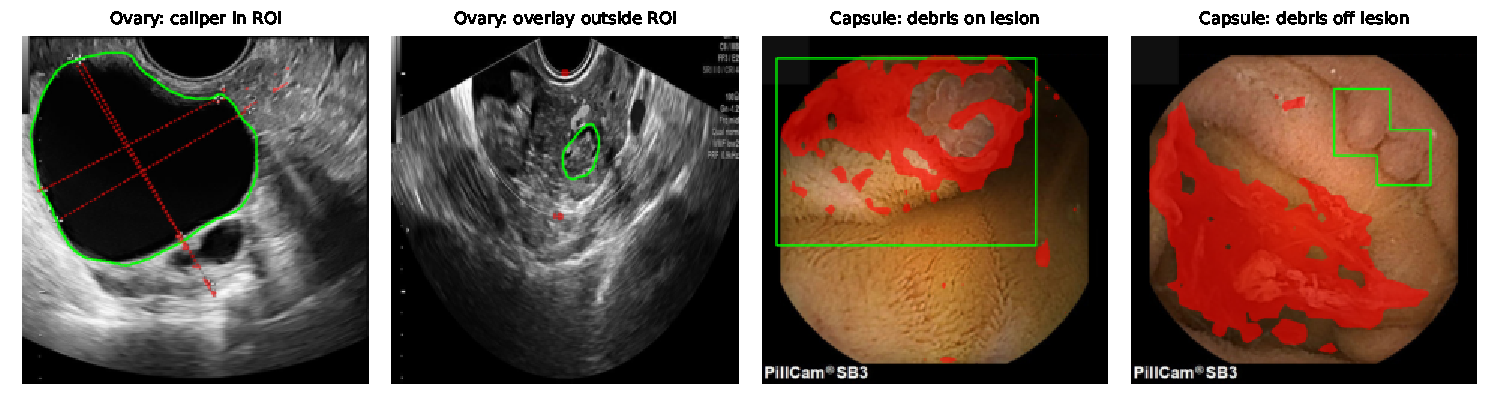
\includegraphics[width=\linewidth]{../../paper/figures/examples.pdf}
\caption{Further real examples with the automatic masks: ovarian calipers crossing the tumour and an overlay outside
it; capsule debris on and off the lesion boxes (MMOTU, SEE-AI; CC BY 4.0).}\label{s3:fig:ex2}\end{figure}
\paragraph{Mask validity} Table~\ref{s3:tab:det}. Lesion masks are accurate (U-Net held-out Dice \sThreeUnetDice; against
HAM manual masks \sThreeUnetHam). The capsule probe reaches pixel accuracy \sThreeProbeAcc{} and IoU \sThreeProbeIoU{}
against held-out expert masks. The thyroid detector's detections lie on a real caliper in 38 of 40 audited images, and
38--39 of 40 caliper-free images are clean. For the ovary, every detection is an on-screen overlay but only 31 of 40
are calipers (the others are dotted zoom arcs and focus markers), and the ``marker-free'' group is caliper-free but not
overlay-free. The morphological hair detector of the pilot is poor (IoU \sThreeHairDetIoU), which is why the hair traps
use the published masks.
\paragraph{Why label noise cannot create the result} An image mislabelled as artifact-bearing (or artifact-free)
weakens the constructed association between $A$ and $Y$ equally in both traps; it biases every effect toward zero. To
create a crossover, errors would have to depend on location \emph{and} on the label, which none of the detectors uses.
\begin{table}[H]\centering\scriptsize
\caption{Validity of the automatic masks that define artifact presence and location. Visual audits: \texttt{docs/ARTIFACT\_MASK\_AUDIT.md} and \texttt{docs/THYROID\_MARKER\_AUDIT.md} (visual audits during the analysis, not by a clinician).}\label{s3:tab:det}
\begin{tabular}{p{3.0cm}p{3.0cm}p{3.8cm}p{4.6cm}}\toprule
Mask & Source & Check & Result \\\midrule
ISIC 2019 lesion masks (BCN, MSK) & U-Net trained on ISIC 2018 Task 1 & held-out Dice (mean) / Dice vs HAM manual masks & 0.886 / 0.895 \\
Hair (DullRazor-type detector, E10) & morphological & IoU / precision / recall vs Mendeley masks & 0.222 / 0.316 / 0.472 \\
Capsule debris masks & patch-token probe (2,160 expert-masked frames) & held-out pixel accuracy / IoU & 0.922 / 0.625 \\
Thyroid (TN3K), detected (A1) & visual audit, 40 images & detection lies on a real caliper / measurement mark & 38/40 (95 \%); 2 border false positives; 1 dotted zoom box (overlay) \\
Thyroid, marker-free (A0) & visual audit, 40 images & no visible caliper & 38–39/40 (95–97 \%); depth-scale ticks present in all images (not label-related) \\
Ovary (MMOTU), detected (A1) & visual audit, 40 images & an on-screen overlay is present & 40/40; caliper specifically 31/40 (others: dotted zoom arcs, focus markers, thumbnail inset) \\
Ovary, marker-free (A0) & visual audit, 40 images & no visible caliper & 37/40 (92 \%) \\
Ovary, marker-free (A0) & visual audit, 40 images & no overlay of any kind (arrows, boxes) & $\sim$29/40 (72 \%); text labels common \\
\bottomrule\end{tabular}
\end{table}


\subsubsection{The crossover with real artifacts}
Table~\ref{s3:tab:traps} and Figure~\ref{s3:fig:forest}. With DINOv2, masking is worth less for in-ROI artifacts in every
cohort:
\begin{itemize}[leftmargin=*]\itemsep1pt
\item \textbf{Dermoscopy hair.} Masking \emph{harms} when the hair lies on the lesion (\sThreeAisicDINOvTwo) and helps
when it lies outside (\sThreeBisicDINOvTwo); crossover \sThreeXisicDINOvTwo{} (as in Stage~1). After masking the Trap-A
model still separates the correlated test (\sThreeMaskCorrAisicDINOvTwo) far better than the reversed one
(\sThreeMaskRevAisicDINOvTwo).
\item \textbf{Thyroid calipers.} Masking helps in both traps but far more when the calipers lie outside the nodule
(\sThreeBthyroidDINOvTwo{} versus \sThreeAthyroidDINOvTwo; crossover \sThreeXthyroidDINOvTwo). In Trap~A the masked model
remains caliper-driven: correlated \sThreeAucThyroidtrapAmaskCorr, reversed \sThreeAucThyroidtrapAmaskRev{}
(Table~\ref{s3:tab:aucenv}); in Trap~B masking removes the gap (\sThreeAucThyroidtrapBmaskCorr{} versus
\sThreeAucThyroidtrapBmaskRev).
\item \textbf{Ovarian calipers.} Crossover \sThreeXovaryDINOvTwo{} (Trap~A \sThreeAovaryDINOvTwo, Trap~B
\sThreeBovaryDINOvTwo).
\item \textbf{Capsule debris.} The largest crossover (\sThreeXcapsuleDINOvTwo): masking recovers almost all of the
reversed-test loss when the debris lies outside the lesion boxes (\sThreeBcapsuleDINOvTwo) and little when it lies on
them (\sThreeAcapsuleDINOvTwo).
\end{itemize}
\paragraph{Other encoder families} The crossover replicates with MedSigLIP (thyroid \sThreeXthyroidMedSigLIP, ovary
\sThreeXovaryMedSigLIP, capsule \sThreeXcapsuleMedSigLIP) and with the CNN ConvNeXt (thyroid \sThreeXthyroidConvNeXt,
capsule \sThreeXcapsuleConvNeXt). With ConvNeXt, masking is useless inside the nodule (\sThreeAthyroidConvNeXt) and
strongly helpful outside it (\sThreeBthyroidConvNeXt). The effect is not a property of vision transformers or of
self-supervised training.
\paragraph{Harm or loss of benefit?} Only for dermoscopy hair does masking actually harm in Trap~A. For calipers and
debris it still helps a little in Trap~A --- it removes clutter and overlays elsewhere on the screen --- but a large
residual shortcut remains. The universal real-data statement is therefore the \emph{crossover}; harm appears where
masking also removes disease context (dermoscopy, and in Stage~2 the controlled sweeps).
\begin{table}[H]\centering\scriptsize
\caption{Real-artifact traps: change in reversed-test AUROC from ROI masking, per trap, and the crossover (5 seeds $\times$ 5 grouped folds; crossed 95\% CIs).}\label{s3:tab:traps}
\resizebox{\linewidth}{!}{\begin{tabular}{lccccc}\toprule
Cohort & Encoder & ERM reversed AUROC A / B & mask $-$ ERM, Trap A (in ROI) & mask $-$ ERM, Trap B (outside) & Crossover B $-$ A \\\midrule
Dermoscopy hair & DINOv2 & 0.510 / 0.510 & $-0.049$ [$-0.083, -0.018$] & $+0.098$ [$+0.060, +0.136$] & $+0.147$ [$+0.111, +0.185$] \\
Dermoscopy hair & DermLIP & 0.665 / 0.735 & $-0.104$ [$-0.143, -0.067$] & $-0.090$ [$-0.135, -0.046$] & $+0.014$ [$-0.037, +0.063$] \\
Thyroid calipers & DINOv2 & 0.289 / 0.405 & $+0.109$ [$+0.085, +0.133$] & $+0.348$ [$+0.307, +0.388$] & $+0.239$ [$+0.196, +0.280$] \\
Thyroid calipers & MedSigLIP & 0.289 / 0.481 & $+0.053$ [$+0.032, +0.073$] & $+0.248$ [$+0.200, +0.293$] & $+0.195$ [$+0.153, +0.238$] \\
Ovarian calipers & DINOv2 & 0.413 / 0.423 & $+0.132$ [$+0.072, +0.196$] & $+0.302$ [$+0.225, +0.378$] & $+0.170$ [$+0.087, +0.252$] \\
Capsule debris & DINOv2 & 0.581 / 0.429 & $+0.084$ [$+0.055, +0.112$] & $+0.461$ [$+0.415, +0.506$] & $+0.377$ [$+0.327, +0.426$] \\
Capsule debris & MedSigLIP & 0.570 / 0.464 & $+0.117$ [$+0.088, +0.147$] & $+0.452$ [$+0.407, +0.495$] & $+0.335$ [$+0.286, +0.383$] \\
Thyroid calipers & ConvNeXt & 0.357 / 0.429 & $-0.004$ [$-0.029, +0.020$] & $+0.271$ [$+0.228, +0.314$] & $+0.275$ [$+0.231, +0.320$] \\
Ovarian calipers & MedSigLIP & 0.426 / 0.551 & $+0.002$ [$-0.048, +0.051$] & $+0.180$ [$+0.120, +0.238$] & $+0.178$ [$+0.109, +0.248$] \\
Capsule debris & ConvNeXt & 0.528 / 0.431 & $+0.084$ [$+0.049, +0.118$] & $+0.403$ [$+0.358, +0.448$] & $+0.320$ [$+0.268, +0.372$] \\
\bottomrule\end{tabular}}
\end{table}

\begin{figure}[H]\centering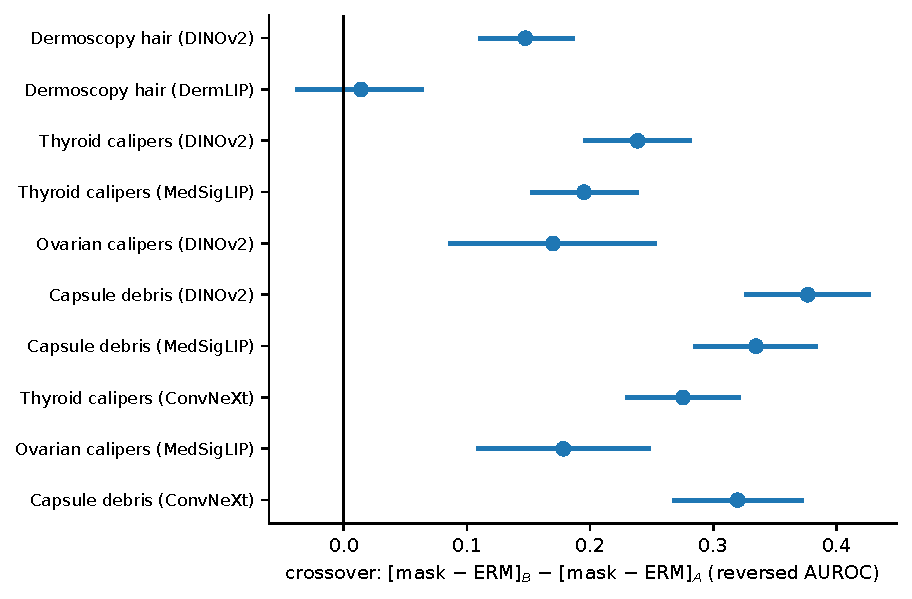
\includegraphics[width=0.78\linewidth]{../stage3_real_artifacts/figures/crossover_forest.pdf}
\caption{Crossover with real artifacts, per cohort and encoder (crossed 95\% CIs).}\label{s3:fig:forest}\end{figure}

\subsubsection{The four location tests}
Table~\ref{s3:tab:primary}. Each cohort's crossover test was registered with the cohort; they are grouped here into one
Holm family. All \sThreeNPOneOK{} of \sThreeNPOne{} are supported ($p\le$ \sThreePMax{} before adjustment).
\begin{table}[H]\centering\small
\caption{The four pre-specified location tests (P1: crossover $>0$), crossed bootstrap, two-sided bootstrap $p$ (floored at $10^{-4}$), Holm-adjusted over the four cohorts.}\label{s3:tab:primary}
\begin{tabular}{lcccc}\toprule
Cohort (DINOv2) & Crossover [95\% CI] & $p$ & $p$ (Holm, 4) & Supported \\\midrule
ISIC hair (DINOv2) & $+0.147$ [$+0.111, +0.185$] & 0.0001 & 0.0004 & \ok \\
Thyroid (DINOv2) & $+0.239$ [$+0.196, +0.280$] & 0.0001 & 0.0004 & \ok \\
Capsule (DINOv2) & $+0.377$ [$+0.327, +0.426$] & 0.0001 & 0.0004 & \ok \\
Ovary (DINOv2) & $+0.170$ [$+0.087, +0.252$] & 0.0001 & 0.0004 & \ok \\
\bottomrule\end{tabular}
\end{table}


\subsubsection{Every arm, and the environments}
Tables~\ref{s3:tab:allarms} and \ref{s3:tab:aucenv}. Three observations matter.
\begin{enumerate}[leftmargin=*]\itemsep1pt
\item \textbf{Label-based methods fix both traps.} Group balancing and DFR, which need image-level artifact labels,
help in both traps of every cohort (e.g.\ thyroid DFR \sThreeArmAThyroiddfr{} in Trap~A), and their benefit does not
depend on location. This replicates the pilot's third claim on three new cohorts.
\item \textbf{Oracle inpainting fails for capsule debris.} Inpainting the debris pixels \emph{lowers} reversed AUROC
(\sThreeArmACapsuleinpaint{} in Trap~A). Erosions carry yellow-white fibrin that resembles debris; inpainting what the
probe calls debris removes disease evidence. Removing artifact pixels is only safe when the artifact does not resemble
the disease.
\item \textbf{Two arms ``help'' by flipping the shortcut.} Unpaired LEACE and prevalence calibration show the largest
reversed-test gains (\sThreeArmAThyroidleaceunpaired, \sThreeArmAThyroidprevcal{} for thyroid), but both remove or
invert the artifact--label association using the artifact label of the \emph{training} set (and prevalence calibration
also at test time), so their correlated AUROC falls far below their reversed one --- the same failure as in Stage~1. They
are reported, not recommended. Paired LEACE, the sound variant, recovers little (thyroid \sThreeArmAThyroidleacepaired).
\end{enumerate}
{\scriptsize
\begin{longtable}{p{2.6cm}p{3.4cm}p{4.0cm}p{4.0cm}}
\caption{Every baseline arm in the real-artifact traps (DINOv2 @518, 5 seeds $\times$ 5 folds): change in reversed-test AUROC versus ERM, crossed 95\% CIs. Inpainting needs the artifact mask; balancing, DFR, unpaired LEACE and prevalence calibration need image-level artifact labels (prevalence calibration also at test time).}\label{s3:tab:allarms}\\\toprule
Cohort & Arm $-$ ERM & Trap A (in ROI) & Trap B (outside) \\\midrule
\endfirsthead
\toprule Cohort & Arm $-$ ERM & Trap A (in ROI) & Trap B (outside) \\\midrule
\endhead
\bottomrule
\endlastfoot
Dermoscopy hair & masking & $-0.049$ [$-0.083, -0.018$] & $+0.098$ [$+0.060, +0.136$] \\
 & oracle inpainting & $+0.098$ [$+0.084, +0.112$] & $+0.100$ [$+0.083, +0.117$] \\
 & group-balanced & $+0.213$ [$+0.183, +0.243$] & $+0.204$ [$+0.166, +0.245$] \\
 & DFR & $+0.196$ [$+0.157, +0.235$] & $+0.196$ [$+0.147, +0.251$] \\
 & paired LEACE & $+0.074$ [$+0.062, +0.086$] & $+0.078$ [$+0.059, +0.097$] \\
 & unpaired LEACE & $+0.320$ [$+0.280, +0.361$] & $+0.295$ [$+0.253, +0.336$] \\
 & prevalence calibration & $+0.415$ [$+0.377, +0.455$] & $+0.429$ [$+0.391, +0.466$] \\
Thyroid calipers & masking & $+0.109$ [$+0.085, +0.133$] & $+0.348$ [$+0.307, +0.388$] \\
 & oracle inpainting & $+0.102$ [$+0.092, +0.112$] & $+0.039$ [$+0.025, +0.053$] \\
 & group-balanced & $+0.388$ [$+0.360, +0.418$] & $+0.254$ [$+0.218, +0.292$] \\
 & DFR & $+0.463$ [$+0.436, +0.492$] & $+0.312$ [$+0.262, +0.362$] \\
 & paired LEACE & $+0.052$ [$+0.045, +0.059$] & $+0.023$ [$+0.014, +0.032$] \\
 & unpaired LEACE & $+0.515$ [$+0.491, +0.538$] & $+0.338$ [$+0.302, +0.375$] \\
 & prevalence calibration & $+0.602$ [$+0.580, +0.625$] & $+0.501$ [$+0.463, +0.538$] \\
Ovarian calipers & masking & $+0.132$ [$+0.072, +0.196$] & $+0.302$ [$+0.225, +0.378$] \\
 & oracle inpainting & $+0.160$ [$+0.135, +0.186$] & $+0.046$ [$+0.032, +0.061$] \\
 & group-balanced & $+0.290$ [$+0.248, +0.332$] & $+0.256$ [$+0.190, +0.320$] \\
 & DFR & $+0.310$ [$+0.263, +0.357$] & $+0.278$ [$+0.209, +0.349$] \\
 & paired LEACE & $+0.142$ [$+0.119, +0.166$] & $+0.031$ [$+0.020, +0.043$] \\
 & unpaired LEACE & $+0.369$ [$+0.320, +0.418$] & $+0.305$ [$+0.230, +0.375$] \\
 & prevalence calibration & $+0.514$ [$+0.468, +0.561$] & $+0.507$ [$+0.440, +0.571$] \\
Capsule debris & masking & $+0.084$ [$+0.055, +0.112$] & $+0.461$ [$+0.415, +0.506$] \\
 & oracle inpainting & $-0.172$ [$-0.202, -0.142$] & $-0.115$ [$-0.144, -0.087$] \\
 & group-balanced & $+0.179$ [$+0.150, +0.205$] & $+0.244$ [$+0.216, +0.272$] \\
 & DFR & $+0.234$ [$+0.199, +0.273$] & $+0.287$ [$+0.239, +0.335$] \\
 & paired LEACE & $+0.012$ [$+0.004, +0.020$] & $+0.010$ [$+0.001, +0.024$] \\
 & unpaired LEACE & $+0.282$ [$+0.247, +0.316$] & $+0.416$ [$+0.374, +0.457$] \\
 & prevalence calibration & $+0.347$ [$+0.316, +0.376$] & $+0.465$ [$+0.430, +0.498$] \\
\end{longtable}}

{\scriptsize
\begin{longtable}{lccccc}
\caption{AUROC of ERM, masking, balancing and DFR in the three test environments (DINOv2, mean over 5 seeds). A large correlated$-$reversed gap is reliance on the artifact.}\label{s3:tab:aucenv}\\\toprule
Cohort & Trap & Arm & clean & correlated & reversed \\\midrule
\endfirsthead
\toprule Cohort & Trap & Arm & clean & correlated & reversed \\\midrule
\endhead
\bottomrule
\endlastfoot
Dermoscopy hair & Trap A & erm & 0.734 & 0.920 & 0.510 \\
 & Trap A & mask & 0.712 & 0.917 & 0.460 \\
 & Trap A & balanced & 0.785 & 0.850 & 0.722 \\
 & Trap A & dfr & 0.715 & 0.740 & 0.705 \\
 & Trap B & erm & 0.716 & 0.894 & 0.510 \\
 & Trap B & mask & 0.701 & 0.795 & 0.608 \\
 & Trap B & balanced & 0.752 & 0.800 & 0.714 \\
 & Trap B & dfr & 0.683 & 0.669 & 0.706 \\
Thyroid calipers & Trap A & erm & 0.608 & 0.879 & 0.289 \\
 & Trap A & mask & 0.689 & 0.908 & 0.398 \\
 & Trap A & balanced & 0.717 & 0.757 & 0.677 \\
 & Trap A & dfr & 0.708 & 0.669 & 0.752 \\
 & Trap B & erm & 0.600 & 0.789 & 0.405 \\
 & Trap B & mask & 0.767 & 0.785 & 0.752 \\
 & Trap B & balanced & 0.657 & 0.660 & 0.659 \\
 & Trap B & dfr & 0.653 & 0.582 & 0.716 \\
Ovarian calipers & Trap A & erm & 0.635 & 0.826 & 0.413 \\
 & Trap A & mask & 0.690 & 0.828 & 0.545 \\
 & Trap A & balanced & 0.710 & 0.725 & 0.703 \\
 & Trap A & dfr & 0.708 & 0.689 & 0.723 \\
 & Trap B & erm & 0.636 & 0.815 & 0.423 \\
 & Trap B & mask & 0.733 & 0.752 & 0.725 \\
 & Trap B & balanced & 0.694 & 0.710 & 0.679 \\
 & Trap B & dfr & 0.671 & 0.632 & 0.701 \\
Capsule debris & Trap A & erm & 0.796 & 0.941 & 0.581 \\
 & Trap A & mask & 0.860 & 0.972 & 0.665 \\
 & Trap A & balanced & 0.847 & 0.916 & 0.760 \\
 & Trap A & dfr & 0.842 & 0.866 & 0.816 \\
 & Trap B & erm & 0.714 & 0.922 & 0.429 \\
 & Trap B & mask & 0.932 & 0.962 & 0.890 \\
 & Trap B & balanced & 0.784 & 0.879 & 0.673 \\
 & Trap B & dfr & 0.762 & 0.819 & 0.716 \\
\end{longtable}}


\subsubsection{What carries the hair shortcut?}
Hair presence and location go with patient and body site (Table~\ref{s3:tab:hairmeta}): in HAM, hair-free lesions are
more often from women and from the lower extremity; in BCN, in-lesion hair goes with older patients and the head and
neck. Two diagnostics show that the hair shortcut is largely carried by these correlates rather than by hair pixels:
\begin{itemize}[leftmargin=*]\itemsep1pt
\item \textbf{Pixel share.} Removing the hair pixels at test time only (oracle inpainting of the ERM model's test
images) closes \sThreePixShareA\% (Trap~A) and \sThreePixShareB\% (Trap~B) of ERM's clean$-$reversed gap: more than
half of what ERM exploits is not in the hair pixels.
\item \textbf{Oracle inpainting} gains about \sThreeArmADermoscopyinpaint{} in Trap~A, half of what balancing gains
(\sThreeArmADermoscopybalanced), which removes the association for hair and everything correlated with it.
\end{itemize}
Two archived sensitivity designs point the same way (\textbf{point estimates, not re-estimated}): an
author-independent reconstruction of the traps (strictly hair-free comparison group, artifact-free clean test) gives a
crossover of \sThreeHdreconcrossover{} but \emph{no} Trap-A harm (\sThreeHdreconmaskminusermtrapA); traps matched on site,
sex and age band give \sThreeHdmetamatchedcrossover{} (Trap~A \sThreeHdmetamatchedmaskminusermtrapA). The crossover is
robust to these choices; the in-lesion harm depends on including lightly haired images and on the strict hair-free
group. Hair is therefore the \emph{correlate-carried} regime: masking cannot remove a shortcut that is carried by who
the patient is and where the lesion is.
\begin{table}[H]\centering\scriptsize
\caption{Patient and site metadata of the hair groups (ISIC 2019): hair presence and location go with age, sex and body site.}\label{s3:tab:hairmeta}
\begin{tabular}{lccccc}\toprule
Source & Group & Mean age & Share female & Share head/neck & Share lower extremity \\\midrule
HAM & hair-free & 57.9 & 0.57 & 0.10 & 0.42 \\
 & Trap A (on lesion) & 52.1 & 0.42 & 0.12 & 0.16 \\
 & Trap B (beside) & 49.9 & 0.45 & 0.14 & 0.26 \\
BCN & hair-free & 61.3 & 0.59 & 0.18 & 0.32 \\
 & Trap A (on lesion) & 58.9 & 0.45 & 0.33 & 0.13 \\
 & Trap B (beside) & 51.8 & 0.45 & 0.22 & 0.18 \\
MSK & hair-free & 51.2 & 0.41 & 0.07 & 0.14 \\
 & Trap A (on lesion) & 54.5 & 0.33 & 0.09 & 0.08 \\
 & Trap B (beside) & 46.9 & 0.45 & 0.09 & 0.11 \\
\bottomrule\end{tabular}
\end{table}

\begin{table}[H]\centering\small
\caption{Dermoscopy hair, Trap A, by image source (DINOv2).}\label{s3:tab:src}
\begin{tabular}{lc}\toprule
Source & mask $-$ ERM, Trap A \\\midrule
HAM & $-0.011$ [$-0.064, +0.043$] \\
BCN & $-0.067$ [$-0.110, -0.025$] \\
\bottomrule\end{tabular}
\end{table}

\paragraph{Hair area relative to the lesion} In Trap~A the in-lesion hair covers a median \sThreeHairRatioMedian{} of
the lesion's area --- similar to the synthetic ruler of Stages~1--2. Masking harms in every tertile of that ratio
(Table~\ref{s3:tab:ratio}); unlike the synthetic sweep, no gradient is visible --- consistent with a shortcut that is not
mainly in the hair pixels.
\begin{table}[H]\centering\small
\caption{Dermoscopy hair, Trap A, by the ratio of in-lesion hair area to lesion area.}\label{s3:tab:ratio}
\begin{tabular}{lcc}\toprule
Hair/lesion area tertile & Median ratio & mask $-$ ERM, Trap A \\\midrule
tertile 1 & 0.006 & $-0.057$ [$-0.095, -0.022$] \\
tertile 2 & 0.033 & $-0.046$ [$-0.082, -0.013$] \\
tertile 3 & 0.113 & $-0.037$ [$-0.071, -0.005$] \\
\bottomrule\end{tabular}
\end{table}


\subsubsection{The exception among encoders: DermLIP}
With DermLIP masking harms at \emph{both} hair locations (Trap~A \sThreeAisicDermLIP, Trap~B \sThreeBisicDermLIP) and the
crossover vanishes (\sThreeXisicDermLIP). DermLIP was trained on whole dermatology images and loses disease signal when
the background is removed, whatever the hair does (Stage~1: clean AUROC falls with masking in both traps).

\subsubsection{Chest radiography: the boundary}
\paragraph{Device traps} Table~\ref{s3:tab:cxr}. With the registered primary encoder RAD-DINO, lung masking helped for both
device types in all four findings (X1 in \sThreeCxrXOneRADDINO{} of 4); neither the in-lung penalty (X2) nor the
crossover (X3) was supported (crossovers \sThreeCxrXminRADDINO{} to \sThreeCxrXmaxRADDINO; in the archived per-seed
analysis one finding, atelectasis, had passed X3). With the registered replication encoder MedSigLIP, fitted for the
first time when these runs were regenerated, the crossover is positive for all four findings (\sThreeCxrXminMedSigLIP{}
to \sThreeCxrXmaxMedSigLIP, Holm), and for effusion masking harms inside the lungs (\sThreeCxrMedSigLIPEffA). The two
encoders differ in what they use: MedSigLIP relies heavily on the out-of-lung tube, which masking removes (Trap~B gains
of 0.23--0.31), whereas RAD-DINO barely uses extra-pulmonary tubes (the synthetic-tube sweep of Stage~2). A confound noted
before the follow-up was fitted: the catheter-free group carries many more out-of-lung tubes than the catheter group
(endotracheal tubes 77\% versus 39\%, nasogastric tubes 83\% versus 42\%), because CLiP's catheter-free images were
selected for other devices; masking removes those tubes, which inflates masking's gain in Trap~A and so works against a
positive crossover. A RAD-DINO follow-up matched within label on view and on the presence of the other devices
(Infiltration) still shows no crossover (Trap~A \sThreeDmtrapA, Trap~B \sThreeDmtrapB, crossover \sThreeDmcrossover;
archived point estimates, \textbf{not re-estimated}). The registered DINOv2 replication was not run.
\begin{table}[H]\centering\scriptsize
\caption{Chest radiographs with real devices (NIH ChestX-ray14 linked to RANZCR-CLiP, AP films): Trap A = central venous catheter inside the lungs, Trap B = endotracheal tube outside them; reversed-test AUROC, crossed 95\% CIs, Holm over the four findings per encoder. Registered claims: X1 masking helps in Trap B, X2 masking harms in Trap A, X3 crossover $>0$. RAD-DINO is the registered primary encoder; the registered MedSigLIP replication was fitted for the first time when these runs were regenerated.}\label{s3:tab:cxr}
\resizebox{\linewidth}{!}{\begin{tabular}{lcccccc}\toprule
Encoder & Finding & mask $-$ ERM, Trap A (in lungs) & mask $-$ ERM, Trap B (outside) & Crossover & $p$ (Holm, 4) & Supported \\\midrule
RAD-DINO & Atelectasis & $+0.059$ [$+0.019, +0.099$] & $+0.105$ [$+0.092, +0.117$] & $+0.046$ [$+0.011, +0.082$] & 0.0544 & X1 \\
 & Consolidation & $+0.074$ [$+0.025, +0.125$] & $+0.070$ [$+0.047, +0.092$] & $-0.004$ [$-0.065, +0.058$] & 0.9112 & X1 \\
 & Effusion & $+0.078$ [$+0.032, +0.125$] & $+0.100$ [$+0.089, +0.111$] & $+0.022$ [$-0.030, +0.074$] & 0.8364 & X1 \\
 & Infiltration & $+0.087$ [$+0.060, +0.116$] & $+0.063$ [$+0.055, +0.071$] & $-0.025$ [$-0.055, +0.006$] & 0.3444 & X1 \\
MedSigLIP & Atelectasis & $+0.183$ [$+0.146, +0.220$] & $+0.278$ [$+0.261, +0.296$] & $+0.095$ [$+0.053, +0.137$] & 0.0004 & X1 X3 \\
 & Consolidation & $+0.087$ [$+0.031, +0.142$] & $+0.226$ [$+0.206, +0.246$] & $+0.139$ [$+0.081, +0.197$] & 0.0004 & X1 X3 \\
 & Effusion & $-0.084$ [$-0.125, -0.043$] & $+0.244$ [$+0.230, +0.259$] & $+0.328$ [$+0.287, +0.369$] & 0.0004 & X1 X2 X3 \\
 & Infiltration & $+0.174$ [$+0.128, +0.219$] & $+0.309$ [$+0.293, +0.325$] & $+0.135$ [$+0.084, +0.185$] & 0.0004 & X1 X3 \\
\bottomrule\end{tabular}}
\end{table}

\paragraph{Chest drains} Table~\ref{s3:tab:drains}. The drain is an extreme shortcut: ERM's reversed AUROC is
\sThreeDrRADDINOermRev{} (RAD-DINO) and \sThreeDrDINOvTwoermRev{} (DINOv2), against clean \sThreeDrRADDINOermClean{} and
\sThreeDrDINOvTwoermClean. Lung masking barely helps (\sThreeDrRADDINOmaskRev, \sThreeDrDINOvTwomaskRev; gain over ERM
\sThreeDrRADDINOMaskGain{} and \sThreeDrDINOvTwoMaskGain), because the drain lies in the lungs. Label-based DFR is best (\sThreeDrRADDINOdfrRev, \sThreeDrDINOvTwodfrRev): a drain comes with a treated,
re-expanded lung, so the shortcut is carried by the treatment's consequences, not only by the tube --- a second
correlate-carried case.
\begin{table}[H]\centering\scriptsize
\caption{Real chest drains (NIH ChestX-ray14 pneumothorax, 29,687 images, patient-grouped folds; drains lie inside the lungs, so this is an in-ROI trap only). AUROC, mean over 5 seeds of 5 patient-grouped folds.}\label{s3:tab:drains}
\begin{tabular}{lcccc}\toprule
Encoder & Arm & clean & correlated & reversed \\\midrule
RAD-DINO & ERM & 0.888 & 0.946 & 0.194 \\
 & lung masking & 0.873 & 0.947 & 0.232 \\
 & group-balanced & 0.858 & 0.880 & 0.540 \\
 & DFR & 0.802 & 0.758 & 0.666 \\
 & masking + DFR & 0.802 & 0.779 & 0.635 \\
DINOv2 & ERM & 0.822 & 0.920 & 0.284 \\
 & lung masking & 0.833 & 0.931 & 0.289 \\
 & group-balanced & 0.786 & 0.846 & 0.402 \\
 & DFR & 0.771 & 0.806 & 0.537 \\
 & masking + DFR & 0.788 & 0.828 & 0.561 \\
\bottomrule\end{tabular}
\end{table}

\paragraph{Reading} Together with the synthetic-tube sweep of Stage~2 (RAD-DINO ignores an out-of-lung tube), chest
radiography is a boundary: in-lung devices are confounded with other devices or carried by correlates, and the
radiograph encoder does not use extra-pulmonary tubes at all. A general medical encoder that does use them (MedSigLIP)
shows the crossover, which is consistent with the law, but one encoder with a confounded contrast is not enough to count
chest radiography as a fifth confirmation; it is reported as a boundary case.

\subsubsection{Datasets considered and not used}
\begin{table}[H]\centering\scriptsize
\caption{Cohorts evaluated for a real-artifact trap and rejected, with the reason (decided before any model was fitted on
them).}\label{s3:tab:rejected}
\begin{tabular}{p{3.4cm}p{2.6cm}p{9.2cm}}\toprule
Dataset & Artifact & Reason \\\midrule
Breast ultrasound (BUSI, BUS-BRA), attempt 1 & calipers & the thyroid detector misses GE-style ``x'' calipers; a two-detector design left the artifact-free group only $\approx$70\% pure on audit \\
Breast ultrasound, attempt 2 & calipers & a patch-token caliper probe (AUROC 0.98 on thyroid/ovary) found only 19 of 2,522 images free of on-screen markings: no artifact-free group exists \\
CANDID-PTX & chest drains & access not granted \\
CXR cardiomegaly lines & lines & too few labelled images \\
TCGA / GrandQC pathology & pen marks & pen masks unreliable \\
ISIC ink & ink marks & ink on the lesion in only 70 images \\
EAD endoscopy & specular reflections & no disease labels \\
BKAI-IGH NeoPolyp colonoscopy & specular highlights & no specular-free images (0), 41 in-polyp \\
DINOv3 encoder & --- & weights gated, access refused \\
\bottomrule\end{tabular}\end{table}

\subsubsection{Sensitivity to the interval estimator}
On the traps of this stage (Table~\ref{s3:tab:estcheck}) the crossed intervals are wider by a median factor of
\sThreeEstMed; \sThreeEstLost{} of \sThreeEstN{} contrasts lose significance and \sThreeEstGained{} gain it
(Table~\ref{s3:tab:estchanges}); none of them is a crossover or a masking effect on the reversed test.
\begin{table}[H]\centering\scriptsize
\caption{Real-artifact traps of the new cohorts under the per-seed and the crossed estimator (same predictions; baseline arms only).}\label{s3:tab:estcheck}
\begin{tabular}{p{5.0cm}p{1.4cm}p{2.6cm}p{2.6cm}p{2.4cm}}\toprule
Result group & Intervals & Excluded 0 only with the per-seed estimator & Excluded 0 only with the crossed estimator & Median width ratio (crossed / per-seed) \\\midrule
capsule/\allowbreak{}convnext384\_universal & 17 & 0 & 0 & 1.38 \\
capsule/\allowbreak{}dino518\_main & 25 & 0 & 1 & 1.59 \\
capsule/\allowbreak{}medsiglip448\_main & 25 & 0 & 0 & 1.69 \\
ovary/\allowbreak{}dino518\_main & 25 & 2 & 0 & 1.67 \\
thyroid/\allowbreak{}convnext384\_universal & 17 & 3 & 0 & 1.68 \\
thyroid/\allowbreak{}dino518\_main & 25 & 1 & 1 & 1.62 \\
thyroid/\allowbreak{}medsiglip448\_main & 25 & 0 & 1 & 1.57 \\
\textbf{all} & 159 & 6 & 3 & 1.62 \\
\bottomrule\end{tabular}
\end{table}

\begin{table}[H]\centering\scriptsize
\caption{Contrasts of the real-artifact traps whose verdict depends on the estimator.}\label{s3:tab:estchanges}
\begin{tabular}{p{4.2cm}p{5.2cm}p{3.3cm}p{2.6cm}}\toprule
Result & Contrast & Crossed estimate [95\% CI] & Verdict vs per-seed estimator \\\midrule
thyroid/\allowbreak{}dino518\_main & trapB /\allowbreak{} dfr /\allowbreak{} clean /\allowbreak{} dfr /\allowbreak{} erm & $+0.053$ [$+0.002, +0.105$] & now excludes 0 \\
thyroid/\allowbreak{}dino518\_main & trapB /\allowbreak{} leace\_paired /\allowbreak{} clean /\allowbreak{} leace\_paired /\allowbreak{} erm & $+0.008$ [$-0.001, +0.018$] & no longer excludes 0 \\
thyroid/\allowbreak{}medsiglip448\_main & trapA /\allowbreak{} inpaint /\allowbreak{} clean /\allowbreak{} inpaint /\allowbreak{} erm & $+0.015$ [$+0.003, +0.025$] & now excludes 0 \\
thyroid/\allowbreak{}convnext384\_universal & trapA /\allowbreak{} mask /\allowbreak{} clean /\allowbreak{} mask /\allowbreak{} erm & $+0.021$ [$-0.000, +0.041$] & no longer excludes 0 \\
thyroid/\allowbreak{}convnext384\_universal & trapB /\allowbreak{} balanced /\allowbreak{} clean /\allowbreak{} balanced /\allowbreak{} erm & $+0.039$ [$-0.002, +0.080$] & no longer excludes 0 \\
thyroid/\allowbreak{}convnext384\_universal & trapB /\allowbreak{} dfr /\allowbreak{} clean /\allowbreak{} dfr /\allowbreak{} erm & $+0.052$ [$-0.001, +0.103$] & no longer excludes 0 \\
ovary/\allowbreak{}dino518\_main & trapB /\allowbreak{} dfr /\allowbreak{} clean /\allowbreak{} dfr /\allowbreak{} erm & $+0.035$ [$-0.018, +0.089$] & no longer excludes 0 \\
ovary/\allowbreak{}dino518\_main & trapB /\allowbreak{} leace\_paired /\allowbreak{} clean /\allowbreak{} leace\_paired /\allowbreak{} erm & $+0.008$ [$-0.000, +0.015$] & no longer excludes 0 \\
capsule/\allowbreak{}dino518\_main & trapB /\allowbreak{} leace\_paired /\allowbreak{} test\_rev /\allowbreak{} leace\_paired /\allowbreak{} erm & $+0.010$ [$+0.001, +0.024$] & now excludes 0 \\
\bottomrule\end{tabular}
\end{table}


\subsection{What failed or changed}
\begin{itemize}[leftmargin=*]\itemsep1pt
\item \textbf{In-ROI masking harms only for dermoscopy hair}; for calipers and debris it helps less. The registered
``harm'' claims (T2, O2, C2) were not supported for thyroid, ovary and capsule.
\item \textbf{DermLIP has no hair crossover}; ``the crossover holds for every encoder'' is not claimed.
\item \textbf{Chest-radiograph device traps}: with RAD-DINO the registered in-ROI penalty was not supported (crossover
in 0 of 4 findings after regeneration, 1 of 4 in the archived analysis); the device-matched follow-up, which was not
regenerated, does not change this. With the MedSigLIP replication it is supported (crossover in 4 of 4, in-lung harm in
1 of 4).
\item \textbf{Oracle inpainting fails on capsule debris}, where the artifact resembles the disease.
\item \textbf{The hair shortcut is mostly correlate-carried}, and the in-lesion harm is sensitive to how the hair-free
group is defined.
\item \textbf{Breast ultrasound was attempted twice and abandoned} (no artifact-free group).
\item \textbf{The artifact masks were audited visually by a non-clinician}; no clinician has checked them yet.
\end{itemize}

\subsection{Anticipated questions}
\paragraph{Why not move the real artifact, as in the sweeps?} A real artifact's position is part of the image. The
two-trap design compares images whose artifact happens to lie inside with images whose artifact lies outside; both are
completed with the same artifact-free images, so the only designed difference is location. That the two groups of
images may differ in other ways is a real limitation of this design.
\paragraph{Why $r\ge0.5$ and $r<0.1$, and what about the images in between?} The thresholds come from the pilot and
leave a gap so that the two traps are clearly separated; the in-between images are used by no trap.
\paragraph{Why does masking still help in Trap~A for calipers and debris?} Ultrasound and capsule frames carry other
on-screen marks and clutter outside the ROI, and removing them helps. What masking cannot do is remove the caliper on
the nodule; the masked Trap-A model's correlated$-$reversed gap stays large.
\paragraph{Why is thyroid benign-heavy in Trap~A?} Calipers are drawn on nodules that are measured, and in this cohort
measured nodules are more often benign; the environments fix the association at 0.9/0.1 whatever the natural rate.
\paragraph{Why are balancing and DFR not simply the answer?} They need image-level artifact labels for every training
image, which clinical datasets rarely have; masking needs only an ROI. They are the reference that shows what is
achievable when labels exist.
\paragraph{Why keep DermLIP if it contradicts the law?} It is a pre-registered replication, and its failure is
informative: an encoder that needs the surroundings of a lesion loses disease signal with any mask, so the comparison
between locations is dominated by that loss.
\paragraph{Why is chest radiography not counted as a confirmation?} In the device traps the in-lung catheter is
confounded with other devices, and in the drain trap the shortcut is carried by the treated lung. Neither isolates
location; counting them either way would be unjustified. The MedSigLIP replication points towards the law, and the
confound works against it, but the primary radiograph encoder shows no crossover, so the evidence is split by encoder.
\paragraph{Is Holm over four tests enough?} The four $p$ values are at the bootstrap floor ($10^{-4}$); any
multiplicity correction over any plausible family leaves them significant.
\paragraph{How reliable are the capsule masks at IoU \sThreeProbeIoU?} Pixel IoU is modest, but the traps use
thresholds on the \emph{fraction} of the frame and of the lesion box covered; small boundary errors move few frames
across 3\% or 10\%. Errors dilute effects rather than create them (Section on mask validity).

\subsection{Conclusion}
\textbf{Supported.} With real artifacts, masking is worth less when the artifact lies inside the ROI: the crossover is
positive in all four cohorts with DINOv2 (Holm over the four location tests), with MedSigLIP in three cohorts and with a
CNN in two. Label-based methods fix both traps. \textbf{Qualified.} Only for dermoscopy hair does masking actually harm
in the in-ROI trap, and that harm depends on how the hair-free group is defined; hair is a correlate-carried shortcut.
\textbf{Not supported.} A crossover with DermLIP; an in-ROI penalty for real chest-radiograph devices with RAD-DINO
(supported with MedSigLIP); pixel removal for
debris that resembles the disease.

\subsection{Questions for the supervisor}
\begin{enumerate}\itemsep1pt
\item Is a visual audit of the automatic artifact masks by a non-clinician acceptable for the thesis, or should a
clinician check a sample before the real-artifact results are written up?
\item Chest radiography now has crossed intervals and a positive MedSigLIP replication (crossover in all four findings)
beside a null primary encoder. Should it stay a boundary case, become a qualified fifth cohort, or move to an appendix?
\item How should the thesis present the correlate-carried nature of the hair shortcut: as a limitation of the hair
cohort, or as a finding about real shortcuts in its own right?
\item Is it acceptable to count calipers and debris as confirmations when masking still helps (less) inside the ROI,
i.e.\ to define the law by the crossover rather than by harm?
\end{enumerate}

